\documentclass[12pt]{report}
\usepackage{tikz}
\usepackage{amsmath}
\pagestyle{plain}




\begin{document}
\author{Andre Gregoire}
\title{CIS770 Homework 1}
\maketitle

\noindent
1. Design a DFA for the language $L_{A1}$ = {w $\in$ \{a,b\}∗\textbar number of a’s in w is not divisible by 3}.

\begin{center}
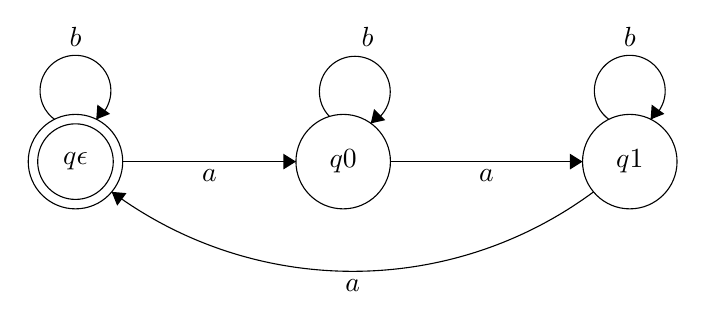
\begin{tikzpicture}[scale=0.2]
\tikzstyle{every node}+=[inner sep=0pt]
\draw [black] (12.2,-16.1) circle (3);
\draw (12.2,-16.1) node {$q\epsilon$};
\draw [black] (12.2,-16.1) circle (2.4);
\draw [black] (29.2,-16.1) circle (3);
\draw (29.2,-16.1) node {$q0$};
\draw [black] (47.4,-16.1) circle (3);
\draw (47.4,-16.1) node {$q1$};
\draw [black] (10.877,-13.42) arc (234:-54:2.25);
\draw (12.2,-8.85) node [above] {$b$};
\fill [black] (13.52,-13.42) -- (14.4,-13.07) -- (13.59,-12.48);
\draw [black] (15.2,-16.1) -- (26.2,-16.1);
\fill [black] (26.2,-16.1) -- (25.4,-15.6) -- (25.4,-16.6);
\draw (20.7,-16.6) node [below] {$a$};
\draw [black] (32.2,-16.1) -- (44.4,-16.1);
\fill [black] (44.4,-16.1) -- (43.6,-15.6) -- (43.6,-16.6);
\draw (38.3,-16.6) node [below] {$a$};
\draw [black] (45.098,-18.021) arc (-53.48909:-126.51091:25.712);
\fill [black] (14.5,-18.02) -- (14.85,-18.9) -- (15.44,-18.1);
\draw (29.8,-23.57) node [below] {$a$};
\draw [black] (28.336,-13.239) arc (224.53768:-63.46232:2.25);
\draw (30.75,-8.85) node [above] {$b$};
\fill [black] (30.95,-13.67) -- (31.87,-13.47) -- (31.16,-12.76);
\draw [black] (46.077,-13.42) arc (234:-54:2.25);
\draw (47.4,-8.85) node [above] {$b$};
\fill [black] (48.72,-13.42) -- (49.6,-13.07) -- (48.79,-12.48);
\end{tikzpicture}
\end{center}

\newpage
\noindent
2.  Design a DFA for the language $L_{A3}$ = {w $\in$ \{a,b\}∗\textbar if w starts with an a then it does not end with a b}.

\begin{center}
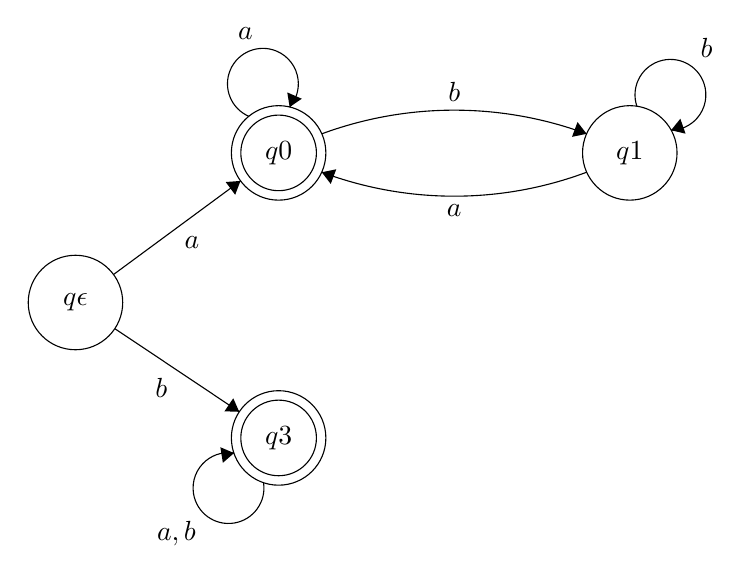
\begin{tikzpicture}[scale=0.2]
\tikzstyle{every node}+=[inner sep=0pt]
\draw [black] (6.5,-21.6) circle (3);
\draw (6.5,-21.6) node {$q\epsilon$};
\draw [black] (19.4,-12.1) circle (3);
\draw (19.4,-12.1) node {$q0$};
\draw [black] (19.4,-12.1) circle (2.4);
\draw [black] (19.4,-30.2) circle (3);
\draw (19.4,-30.2) node {$q3$};
\draw [black] (19.4,-30.2) circle (2.4);
\draw [black] (41.7,-12.1) circle (3);
\draw (41.7,-12.1) node {$q1$};
\draw [black] (22.143,-10.889) arc (110.27614:69.72386:24.26);
\fill [black] (38.96,-10.89) -- (38.38,-10.14) -- (38.03,-11.08);
\draw (30.55,-8.89) node [above] {$b$};
\draw [black] (8.92,-19.82) -- (16.98,-13.88);
\fill [black] (16.98,-13.88) -- (16.04,-13.95) -- (16.64,-14.76);
\draw (13.9,-17.35) node [below] {$a$};
\draw [black] (9,-23.26) -- (16.9,-28.54);
\fill [black] (16.9,-28.54) -- (16.52,-27.68) -- (15.96,-28.51);
\draw (11.95,-26.4) node [below] {$b$};
\draw [black] (38.964,-13.325) arc (-69.46451:-110.53549:23.985);
\fill [black] (22.14,-13.33) -- (22.71,-14.07) -- (23.06,-13.14);
\draw (30.55,-15.35) node [below] {$a$};
\draw [black] (17.516,-9.78) arc (246.80427:-41.19573:2.25);
\draw (17.29,-4.94) node [above] {$a$};
\fill [black] (20.1,-9.19) -- (20.87,-8.66) -- (19.95,-8.26);
\draw [black] (42.153,-9.146) arc (199.00798:-88.99202:2.25);
\draw (46.57,-6.07) node [above] {$b$};
\fill [black] (44.32,-10.66) -- (45.24,-10.88) -- (44.91,-9.93);
\draw [black] (18.44,-33.03) arc (9:-279:2.25);
\draw (12.91,-35.45) node [below] {$a,b$};
\fill [black] (16.57,-31.16) -- (15.7,-30.79) -- (15.86,-31.78);
\end{tikzpicture}
\end{center}

\newpage
\noindent
3.  Design a DFA for the language $L_{A4}$ = {w $\in$ \{a,b\}∗ \textbar \textit{ba} appears exactly twice as a substring}.
\begin{center}
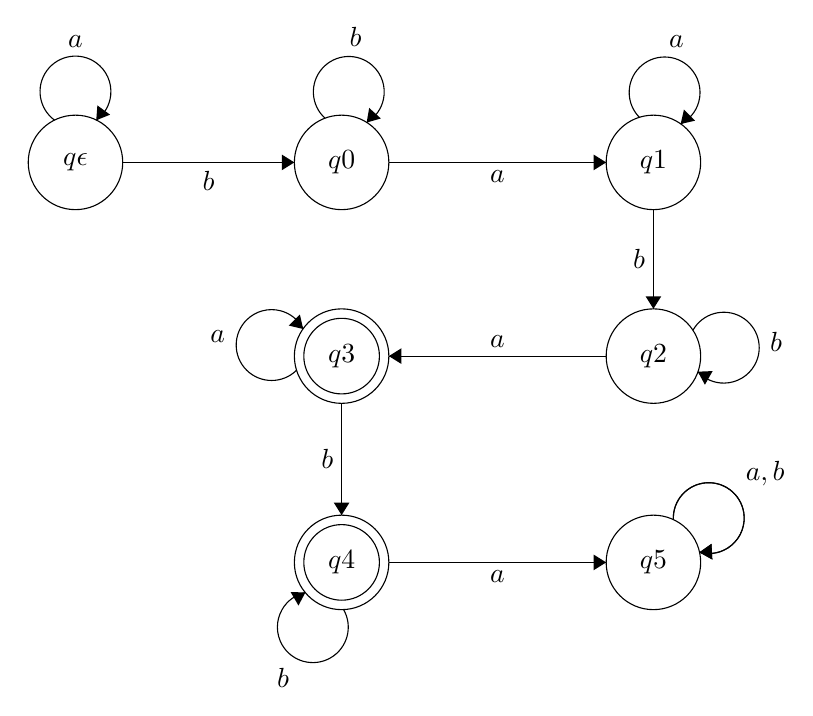
\begin{tikzpicture}[scale=0.2]
\tikzstyle{every node}+=[inner sep=0pt]
\draw [black] (10.5,-10.6) circle (3);
\draw (10.5,-10.6) node {$q\epsilon$};
\draw [black] (27.4,-10.6) circle (3);
\draw (27.4,-10.6) node {$q0$};
\draw [black] (47.2,-10.6) circle (3);
\draw (47.2,-10.6) node {$q1$};
\draw [black] (47.2,-22.9) circle (3);
\draw (47.2,-22.9) node {$q2$};
\draw [black] (27.4,-22.9) circle (3);
\draw (27.4,-22.9) node {$q3$};
\draw [black] (27.4,-22.9) circle (2.4);
\draw [black] (27.4,-36) circle (3);
\draw (27.4,-36) node {$q4$};
\draw [black] (27.4,-36) circle (2.4);
\draw [black] (47.2,-36) circle (3);
\draw (47.2,-36) node {$q5$};
\draw [black] (13.5,-10.6) -- (24.4,-10.6);
\fill [black] (24.4,-10.6) -- (23.6,-10.1) -- (23.6,-11.1);
\draw (18.95,-11.1) node [below] {$b$};
\draw [black] (9.177,-7.92) arc (234:-54:2.25);
\draw (10.5,-3.35) node [above] {$a$};
\fill [black] (11.82,-7.92) -- (12.7,-7.57) -- (11.89,-6.98);
\draw [black] (30.4,-10.6) -- (44.2,-10.6);
\fill [black] (44.2,-10.6) -- (43.4,-10.1) -- (43.4,-11.1);
\draw (37.3,-11.1) node [below] {$a$};
\draw [black] (47.2,-13.6) -- (47.2,-19.9);
\fill [black] (47.2,-19.9) -- (47.7,-19.1) -- (46.7,-19.1);
\draw (46.7,-16.75) node [left] {$b$};
\draw [black] (44.2,-22.9) -- (30.4,-22.9);
\fill [black] (30.4,-22.9) -- (31.2,-23.4) -- (31.2,-22.4);
\draw (37.3,-22.4) node [above] {$a$};
\draw [black] (27.4,-25.9) -- (27.4,-33);
\fill [black] (27.4,-33) -- (27.9,-32.2) -- (26.9,-32.2);
\draw (26.9,-29.45) node [left] {$b$};
\draw [black] (30.4,-36) -- (44.2,-36);
\fill [black] (44.2,-36) -- (43.4,-35.5) -- (43.4,-36.5);
\draw (37.3,-36.5) node [below] {$a$};
\draw [black] (26.356,-7.8) arc (228.18687:-59.81313:2.25);
\draw (28.28,-3.3) node [above] {$b$};
\fill [black] (28.99,-8.07) -- (29.89,-7.81) -- (29.15,-7.14);
\draw [black] (46.317,-7.745) arc (224.90972:-63.09028:2.25);
\draw (48.66,-3.35) node [above] {$a$};
\fill [black] (48.93,-8.16) -- (49.85,-7.95) -- (49.14,-7.24);
\draw [black] (49.703,-21.268) arc (150.84277:-137.15723:2.25);
\draw (54.57,-21.97) node [right] {$b$};
\fill [black] (50.02,-23.89) -- (50.47,-24.72) -- (50.96,-23.85);
\draw [black] (24.547,-23.788) arc (315.02737:27.02737:2.25);
\draw (20.03,-21.64) node [left] {$a$};
\fill [black] (24.96,-21.18) -- (24.75,-20.26) -- (24.04,-20.96);
\draw [black] (27.52,-38.986) arc (30.03751:-257.96249:2.25);
\draw (23.68,-42.68) node [below] {$b$};
\fill [black] (25.1,-37.91) -- (24.16,-37.88) -- (24.66,-38.74);
\draw [black] (48.466,-33.293) arc (182.65981:-105.34019:2.25);
\draw (53.03,-30.36) node [right] {$a,b$};
\fill [black] (50.12,-35.36) -- (50.94,-35.82) -- (50.89,-34.82);
\draw [black] (48.466,-33.293) arc (182.65981:-105.34019:2.25);
\fill [black] (50.12,-35.36) -- (50.94,-35.82) -- (50.89,-34.82);
\end{tikzpicture}
\end{center}


\newpage
\noindent
4. Let $A\textsubscript k \subseteq \{a,b\}$* be the collection of strings \textit w where there is a position \textit i in \textit w such that the symbol at position \textit i (in \textit w) is \textit a, and the symbol at position \textit i + \textit k is \textit b. For example, consider $A \textsubscript 2$ (when \textit k = 2). \textit baab $\in$ $A \textsubscript 2$ because the second position (\textit i = 2) has an\textit a and the fourth position has a\textit b. On the other hand, \textit b\textit b $\notin$ $A \textsubscript 2$ (because there are no \textit as) and \textit aba $\notin$ $A \textsubscript 2$ (because none of the \textit as are followed by a \textit b 2 positions away).
\newline

\noindent
4-1. Design a DFA for language $A\textsubscript k$. Your formal description (by listing states, transitions, etc. and not “drawing the DFA”) will depend on the parameter \textit k but should work no matter what \textit k is; see lecture 2, last page for such an example.
\break \break
\noindent
$M_k\text{ = }(Q, \{a,b\}, \delta, q\textsubscript 0, F)$\break
$\delta (q_\epsilon, a)\text{ = }q_a$\break
$\delta (q_\epsilon, b)\text{ = }q_b$\break
$\delta (q_b, a)\text{ = }q_a$\break
$\delta (q_b, b)\text{ = }q_b$\break
$\delta (q_a, a)\text{ = }q_{aw}$\break
$\delta (q_a, b)\text{ = }q_{aw}$\break
$\text{where }q_{aw}\text{ = }q_{aw} \text{1 ... } q_{aw} \text{k-1}$\break
$\delta (q_{aw}, a)\text{  = }q_{aw}	\text{ if \textbar aw\textbar $<$  k-1 }$\break
$\delta (q_{aw}, b)\text{  = }q_{aw}	 \text{ if \textbar aw\textbar  $<$  k-1  otherwise  } {q_{aw}}_b$\break
$q_0\text{ = }q_\epsilon$\break
$F\text{ = }q_{awb}$\break


\noindent
4-2. Prove that your DFA is correct when \textit k = 2.

Below is a DFA for the K = 2 case

\begin{center}
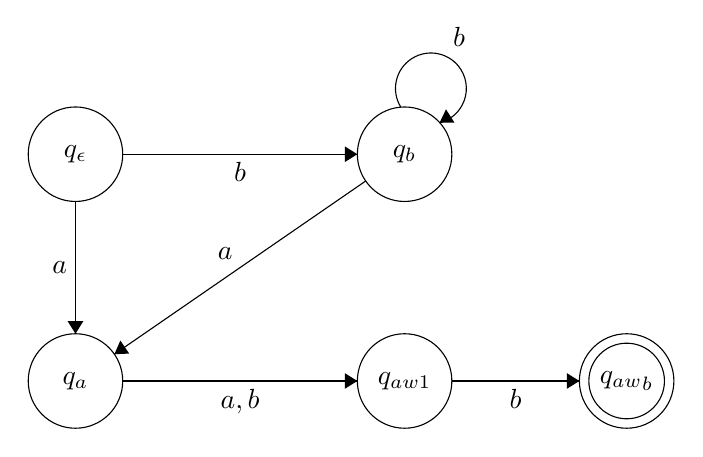
\begin{tikzpicture}[scale=0.2]
\tikzstyle{every node}+=[inner sep=0pt]
\draw [black] (17,-16.6) circle (3);
\draw (17,-16.6) node {$q_\epsilon$};
\draw [black] (37.9,-16.6) circle (3);
\draw (37.9,-16.6) node {$q_b$};
\draw [black] (17,-31) circle (3);
\draw (17,-31) node {$q_a$};
\draw [black] (37.9,-31) circle (3);
\draw (37.9,-31) node {${q_{aw1}}$};
\draw [black] (52,-31) circle (3);
\draw (52,-31) node {${q_{aw}}_b$};
\draw [black] (52,-31) circle (2.4);
\draw [black] (20,-16.6) -- (34.9,-16.6);
\fill [black] (34.9,-16.6) -- (34.1,-16.1) -- (34.1,-17.1);
\draw (27.45,-17.1) node [below] {$b$};
\draw [black] (37.667,-13.621) arc (212.19859:-75.80141:2.25);
\draw (41.36,-9.82) node [above] {$b$};
\fill [black] (40.12,-14.6) -- (41.07,-14.6) -- (40.53,-13.75);
\draw [black] (17,-19.6) -- (17,-28);
\fill [black] (17,-28) -- (17.5,-27.2) -- (16.5,-27.2);
\draw (16.5,-23.8) node [left] {$a$};
\draw [black] (35.43,-18.3) -- (19.47,-29.3);
\fill [black] (19.47,-29.3) -- (20.41,-29.26) -- (19.85,-28.43);
\draw (26.5,-23.3) node [above] {$a$};
\draw [black] (20,-31) -- (34.9,-31);
\fill [black] (34.9,-31) -- (34.1,-30.5) -- (34.1,-31.5);
\draw (27.45,-31.5) node [below] {$a,b$};
\draw [black] (40.9,-31) -- (49,-31);
\fill [black] (49,-31) -- (48.2,-30.5) -- (48.2,-31.5);
\draw (44.95,-31.5) node [below] {$b$};
\end{tikzpicture}
\end{center}

\break
\break
\noindent
$Assume\text{ \textit i = }3\text{ and }\textit K\text{ = }2$\break
$\text{\textbf{Base: }}\textit w\text{ = }\epsilon$\break
$\text{Because \textbar \textit w\textbar = 0 the word is rejected}$\break\break\noindent
$\text{\textbf{Hypothesis: }}$\break
$\textit w\text{ = }ba\textbf abbaaab$\break
$w_i\text{ = }a\text{ noted in bold above}$\break\break

\noindent
If we choose a position i where w[i] = a, it is only neccesary to test the substring w[i] to w[i+k].  Therefore if w[i] is assumed to be the first character read into the DFA the following transition sequence is followed: 
\break
$(q_e, a)\text{ = }a$\break
$(q_a, b)\text{ = }q_{aw1}$\break
$(q_{aw}, b)\text{ = }q_{awb}\text{ because \textbar aw\textbar = k-1}$\break

\noindent
Because we reached the finish state following the set transitions, the DFA holds true.



\end{document}



